\section{Auswertung}
	\label{sec:auswertung}

	F"ur die Leerlaufspannung $U_0$ und den Kurzsschlussstrom $I_K$ ergaben sich die in Tabelle \eqref{tabelle_anfang} gemessenen Werte in Abh"angigkeit vom Lampenabstand.
	Es ist zu erkennen, dass der Kurzschlussstrom $I_K$ bei geringerem Abstand zunimmt, w"ahrend die Leerlaufspannung nahezu konstant bleibt.

	\begin{table}[h]	
\centering
\begin{tabular}{|r||r||r||r|} \hline
Abstand[cm]	&	I_K[mA]	&	U_0[mV]	& Intensit"at[mW/cm^2]\\ \hline
71.8	&	31.4	&	1.942	&	8.76
52.6	&	50.4	&	2	&	14.6
36.7	&	75	&	2.06	&	22.76
29	&	100.5	& 	2.02	&	25.96
\end{tabular}
\caption{Kurzschlussstrom und Leerlaufspannung in Abh"angigkeit vom Lampenabstand}
\label{tabelle_anfang}
\end{table}

	Beim Aufragen von $I_K$ und $U_0$ gegen Intensit"at $J$ ergaben sich die Graphen \eqref{IJ} und \eqref{UJ}.
	Durch lineare Regression des I-J-Graphen ergab sich f"ur den Proportionalit"atsfaktor $\lambda$:\\

	\begin{equation*}
		\lambda = \SI{3.77 (51)}{}
	\end{equation*}

	\begin{figure}[htbp]
		\centering
		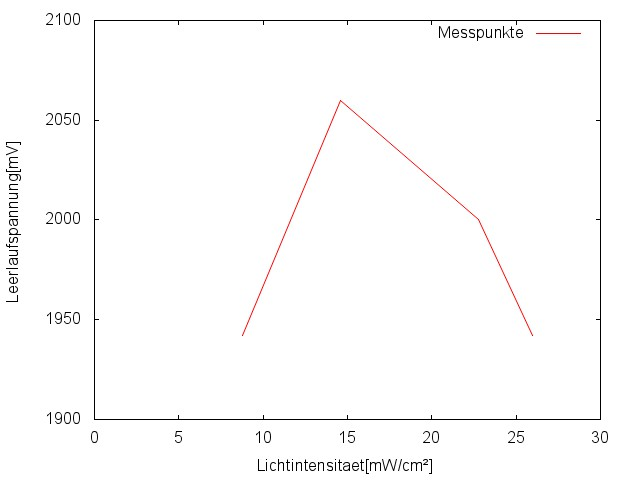
\includegraphics[width = 12cm]{img/UJ.jpg}
		\caption{Leerlaufspannung gegen die Intensit"at aufgetragen}
		\label{UJ}

		
		\centering
		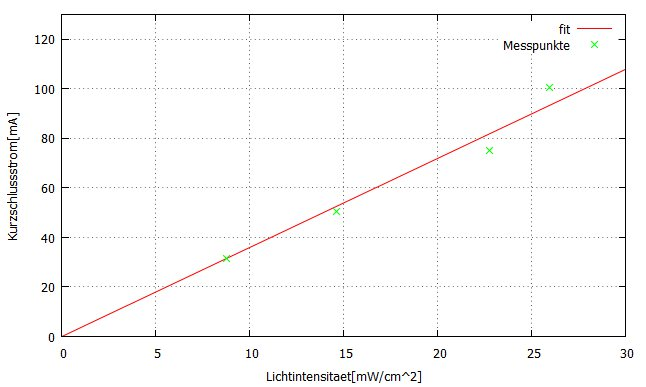
\includegraphics[width = 12cm]{img/IJ.jpg}
		\caption{Kurzschlusstrom gegen die Intensit"at aufgetragen mit linearer Regression}
		\label{IJ}
	\end{figure}

	F"ur die U-I-Kennlinen \eqref{UI1} bis \eqref{UI4} ergab sich eine Diodenkennlinie mit umgekehrtem Vorzeichen.
	Die gelbe Fl"ache gibt dabei die maximale Leistung $P_{max}$ an.\\

	\begin{table}[h]	
\centering
\begin{tabular}{|r||r||r|} \hline
R[\Omega]	&	I[mA]	&	U[mv]	\\ \hline
5	&	98.2	&	715	\\
10	&	97.3	&	1199	\\
11	&	98.7	&	1380	\\
12	&	98.5	&	1480	\\
13	&	98.4	&	1605	\\
14	&	98.0	&	1710	\\
15	&	96.5	&	1795	\\
16	&	94.6	&	1860	\\
17	&	91.7	&	1910	\\
18	&	88.6	&	1949	\\
19	&	85.3	&	1974	\\
20	&	82.4	&	1990	\\
21	&	79.1	&	2020	\\
22	&	76.3	&	2040	\\
23	&	73.5	&	2050	\\
24	&	71.0	&	2060	\\
25	&	68.8	&	2070	\\
26	&	66.6	&	2090	\\
27	&	64.5	&	2090	\\
28	&	62.6	&	2100	\\
29	&	60.7	&	2110	\\
30	&	59.0	&	2120	\\
40	&	45.8	&	2150	\\
50	&	37.2	&	2170	\\
60	&	31.3	&	2190	\\
70	&	27.1	&	2190	\\
80	&	23.8	&	2200	\\
90	&	21.3	&	2210	\\
100	&	19.2	&	2210	\\
\end{tabular}
\caption{Strom und Spannung in Abh"angigkeit vom Widerstand bei einem Abstand von 29cm}
\label{tabelle_290}
\end{table}
	\begin{table}[h]	
\centering
\begin{tabular}{|r||r||r|} \hline
R[\Omega]	&	I[mA]	&	U[mV]	\\ \hline
5	&	76.4	&	539	\\
10	&	76.1	&	600	\\
15	&	76.4	&	700	\\
18	&	76.5	&	773	\\
19	&	77.0	&	848	\\
20	&	75.0	&	1660	\\
21	&	74.1	&	1710	\\
22	&	72.7	&	1748	\\
23	&	70.9	&	1774	\\
24	&	69.1	&	1798	\\
25	&	67.2	&	1815	\\
26	&	65.3	&	1830	\\
27	&	63.3	&	1840	\\
28	&	61.7	&	1850	\\
29	&	60.0	&	1860	\\
30	&	58.4	&	1869	\\
35	&	51.3	&	1897	\\
40	&	45.8	&	1919	\\
50	&	37.5	&	1944	\\
60	&	31.6	&	1958	\\
70	&	27.4	&	1968	\\
80	&	24.1	&	1975	\\
90	&	21.5	&	1980	\\
100	&	19.5	&	1983	\\
200	&	9.9	&	2000	\\
\end{tabular}
\caption{Strom und Spannung in Abh"angigkeit vom Widerstand bei einem Abstand von 36.7cm}
\label{tabelle_367}
\end{table}
	\begin{table}[h]	
\centering
\begin{tabular}{|r||r||r|} \hline
R[\ohm]	&	I[mA]	&	U[mv]	\\ \hline
5	&	50.4	&	439	\\
10	&	50.4 	&	640	\\
15	&	50.4	&	884	\\
20	&	50.4	&	1135	\\
25	&	50.2	&	1378	\\
26	&	48.0	&	1574	\\
27	&	49.7	&	1445	\\
28	&	49.5	&	1483	\\
29	&	48.8	&	1508	\\
30	&	34.7	&	1802	\\
31	&	34.2	&	1809	\\
32	&	33.6	&	1814	\\
33	&	33.1	&	1817	\\
34	&	32.5	&	1821	\\
35	&	44.0	&	1685	\\
40	&	41.0	&	1739	\\
45	&	37.6	&	1784	\\
50	&	34.9	&	1814	\\
55	&	32.3	&	1838	\\
60	&	30.0	&	1857	\\
70	&	26.1	&	1873	\\
80	&	23.1	&	1893	\\
90	&	20.8	&	1908	\\
100	&	18.9	&	1916	\\
200	&	9.7	&	1958	\\
\end{tabular}
\caption{Strom und Spannung in Abh"angigkeit vom Widerstand bei einem Abstand von 52.6cm}
\label{tabelle_526}
\end{table}
	\begin{table}[h]	
\centering
\begin{tabular}{|r||r||r|} \hline
R[\Omega]	&	I[mA]	&	U[mV]	\\ \hline
5	&	31.4	&	219	\\
10	&	31.6	&	377	\\
15	&	31.3	&	534	\\
20	&	31.3	&	686	\\
25	&	31.4	&	841	\\
30	&	31.3	&	1000	\\
35	&	31.3	&	1155	\\
40	&	31.0	&	1298	\\
45	&	30.2 	&	1409	\\
46	&	29.8	&	1420	\\
47	&	29.6	&	1445	\\
48	&	29.3	&	1455	\\
49	&	29.0 	&	1470	\\
50	&	28.7	&	1486	\\
51	&	28.4	&	1500	\\
52	&	28.1	&	1510	\\
53	&	27.9	&	1527	\\
54	&	27.6	&	1540	\\
55	&	27.5	&	1558	\\
60	&	26.0	&	1604	\\
65	&	24.5	&	1638	\\
70	&	23.2	&	1665	\\
75	&	22.0	&	1690	\\
80	&	20.9	&	1709	\\
85	&	19.9	&	1726	\\
90	&	19.0 	&	1742	\\
95	&	18.1	&	1754	\\
100	&	17.4	&	1765	\\
110	&	16.0 	&	1783	\\
120	&	14.8	&	1796	\\
130	&	13.7	&	1807	\\
140	&	12.8	&	1815	\\
150	&	12.0 	&	1825	\\
160	&	11.3	&	1832	\\
170	&	10.7	&	1839	\\
180	&	10.2	&	1845	\\
190	&	09.1	&	1848	\\
200	&	09.2	&	1853	\\
250	&	07.4	&	1870	\\
300	&	06.2	&	1880	\\
\end{tabular}
\caption{Strom und Spannung in Abh"angigkeit vom Widerstand bei einem Abstand von 71.8cm}
\label{tabelle_718}
\end{table}

	\begin{figure}[htbp]
		\centering
		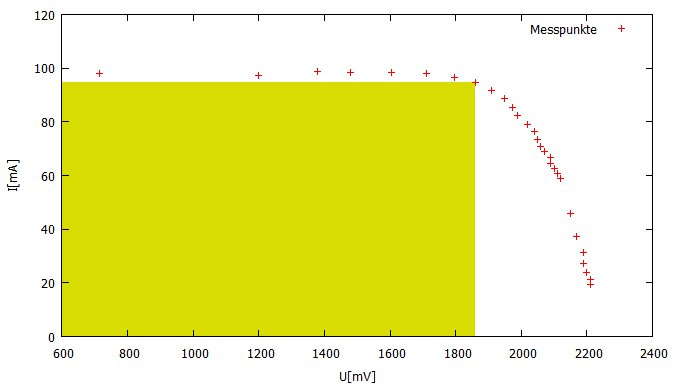
\includegraphics[width = 12cm]{img/290.jpg}
		\caption{Kennlinie bei einem Lampenabstand von 29cm	}
		\label{UI1}

		\centering
		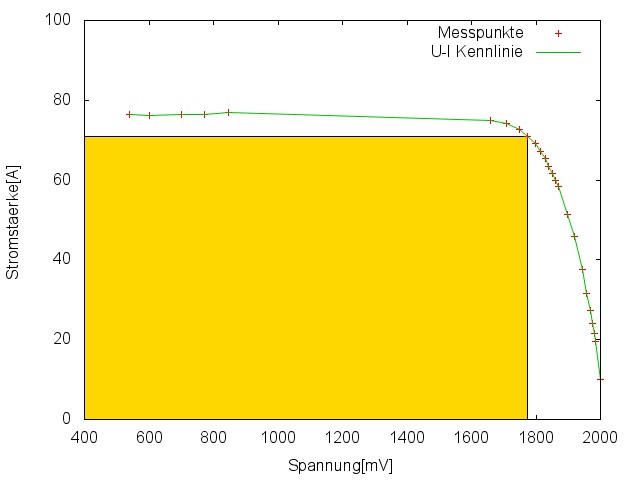
\includegraphics[width = 12cm]{img/367.jpg}
		\caption{Kennlinie bei einem Lampenabstand von 36.7cm}
		\label{UI2}
	\end{figure}
	\begin{figure}[htbp]
		\centering
		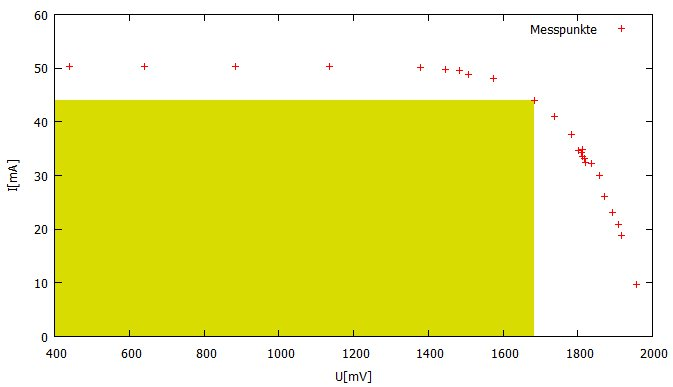
\includegraphics[width = 12cm]{img/526.jpg}
		\caption{Kennlinie bei einem Lampenabstand von 52.6cm}
		\label{UI3}

		\centering
		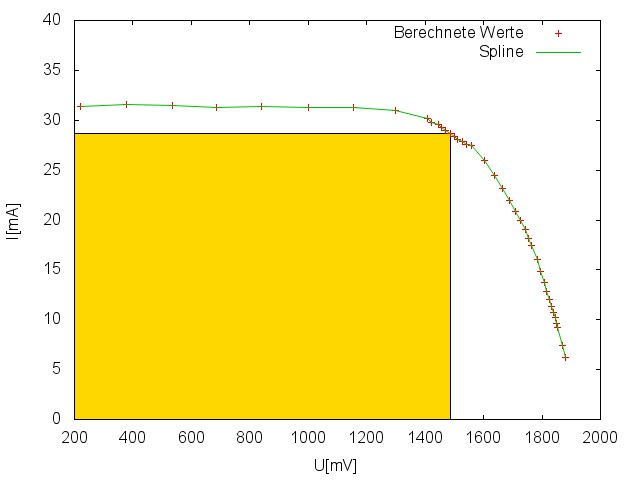
\includegraphics[width = 12cm]{img/718.jpg}
		\caption{Kennlinie bei einem Lampenabstand von 71.8cm}
		\label{UI4}
	\end{figure}

	Die Graphen \eqref{PR1} bis \eqref{PR4} geben die abgegebene Leistung $P$ f"ur unterschiedliche Lastwiderst"ande $R$ an.
	Dabei kann nicht der eingestellte Widerstand benutzt werden, da sich in der Solarzelle noch ein weiterer Leistungsabh"angiger Widerstand befindet.
	Die Leistung ist Widerstandsabh"angig.
	Sie steigt bis zu einem Maximalwert an und f"allt anschlie"send kontinuierlich.
	Dies ist dadurch zu erkl"aren, dass sich die Spannung $U$ langsam $U_0$ ann"ahert, w"ahrend $I_K$ kontinuierlich abf"allt.\\

	\begin{figure}[htbp]
		\centering
		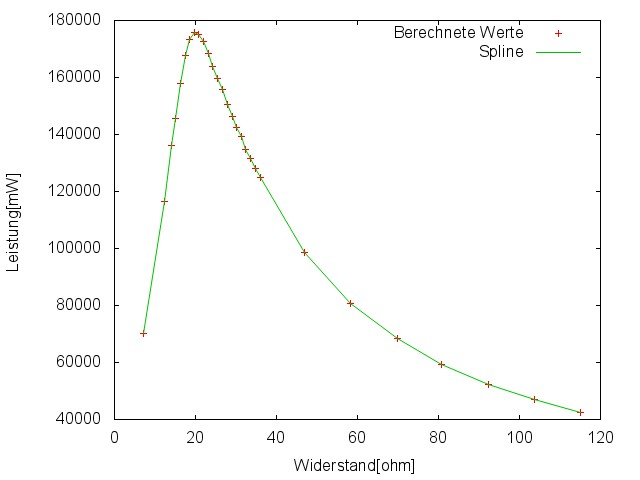
\includegraphics[width = 12cm]{img/290p.jpg}
		\caption{Leistung in Abh"angigkeit des Widerstandes}
		\label{PR1}

		\centering
		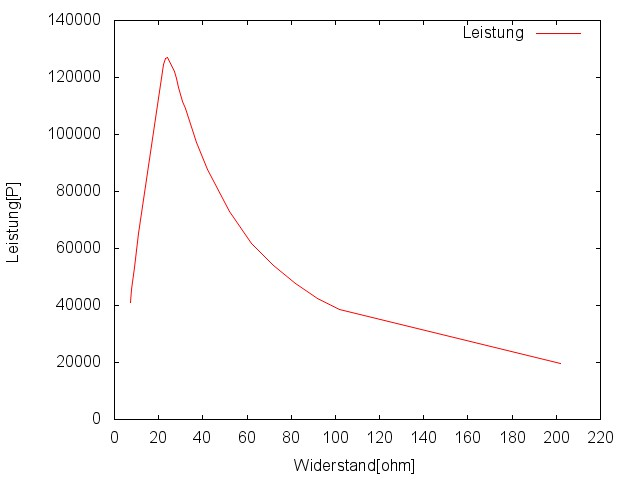
\includegraphics[width = 12cm]{img/367p.jpg}
		\caption{Leistung in Abh"angigkeit des Widerstandes}
		\label{PR2}
\end{figure}
\begin{figure}[htbp]
		\centering
		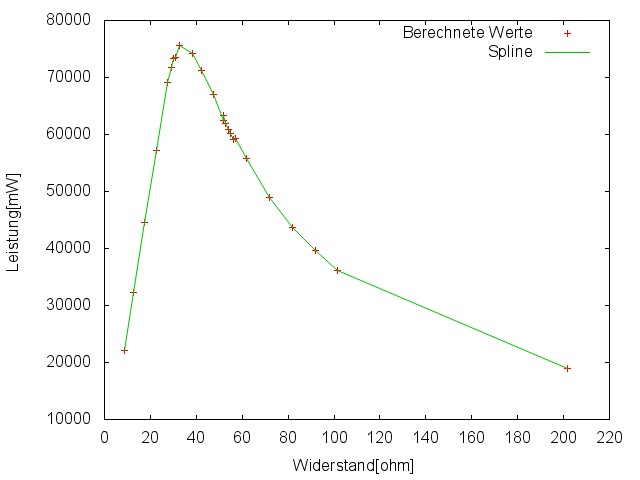
\includegraphics[width = 12cm]{img/526p.jpg}
		\caption{Leistung in Abh"angigkeit des Widerstandes}
		\label{PR3}

		\centering
		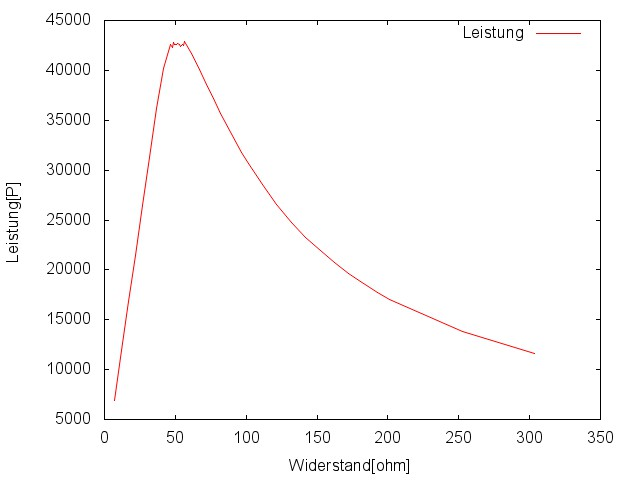
\includegraphics[width = 12cm]{img/718p.jpg}
		\caption{Leistung in Abh"angigkeit des Widerstandes}
		\label{PR4}
	\end{figure}
\newpage
	F"ur den Wirkungsgrad $\eta$ ergibt sich:

	\begin{eqnarray*}
		P_{ein} = A \cdot J\\
		A = \SI{45.6}{\centi\meter^2}\\
		P_{aus} = P_{max}\\
		\Rightarrow \qquad \eta = \frac{P_{max}}{P_{ein}} 
	\end{eqnarray*}

	Der Wirkungsgrad ist daher abh"angig von der Intensit"at des Lichts und der Maximal erbrachten Leistung.
	Eine lineare Regression des Graphen \eqref{wirkung} ergiebt:

	\begin{equation*}
		\eta = \SI{0.161 (20)}{}
	\end{equation*}

	Damit wird der Literaturwert aus \cite{artikel2} von $16\%$ erreicht.\\

	\begin{table}[h]	
\centering
\begin{tabular}{|r||r|} \hline
Abstand[cm]	&	P_max[mW]\\ \hline
71.8	&	42.65
52.6	&	74.14
36.7	&	12.71
29	&	17.60
\end{tabular}
\caption{Maximalleistung in Abh"angigkeit zum Abstand}
\label{tabelle_max}
\end{table}

	\begin{figure}[htbp]
		\centering
		\includegraphics[width = 12cm]{img/wirkung.jpg}
		\caption{$P_{aus}$ gegen $P_{ein}$}
		\label{wirkung}
	\end{figure}